\documentclass[11pt,a4paper]{article}
\usepackage[margin=0.78in]{geometry}
\usepackage[T1]{fontenc}
\usepackage{lmodern,amsmath,amssymb,booktabs,tabularx,xcolor,graphicx}
\usepackage[hidelinks]{hyperref}
\usepackage{enumitem}
\setlist{nosep,leftmargin=*}
\setlength{\parindent}{0pt}
\setlength{\parskip}{4pt}
\newif\ifguidance
\guidancefalse
\newcommand{\help}[1]{\ifguidance{\small\color{blue!55!black}\textit{Writing guide: #1}\par}\fi}
\newcommand{\fillin}[1]{\textnormal{[\textit{#1}]}}
\newcommand{\ProjectTitle}{Local Bayesian-Network Factor Adaptation for Fairness Transfer across States and Years}
\newcommand{\EO}{\Delta_{\mathrm{EOdds}}}
\begin{document}
\begin{center}
{\Large\bfseries \ProjectTitle}\\[4pt]
ICT 5143: Algorithms Fairness and Graphical Models Laboratory\\
Problem 5; Team \fillin{ID}\\
Aslam Mugutkhan, 261090830010; Rao Ashlesha Padmananda, 261090830019\\
{\small Repository: \url{https://example.org/replace-with-repository}\\
Submission commit: \texttt{REPLACE}; Date: 07/11/26}
\end{center}
\begin{abstract}
Can updating at most two shifted Bayesian-network factors preserve equalized odds better than global adaptation when
only 200 or 1,000 target labels are available? On ACSIncome (CA, TX, NY; 2018--2019; nine transfers) we propose BN-LFA:
Bayes-factor $\times$ decision-impact factor selection, then equalized-odds thresholds refitted on source data reweighted
by the selected factors. BN-LFA was fairer than target threshold adjustment (mean $\EO$ $-0.039$ and $-0.065$, Holm
$p=0.006$) and than updating every factor at $n=200$ ($-0.014$, $p=0.032$), but not than covariate reweighting, and not
clearly than keeping the source rule.
\end{abstract}

\section{Question, context and contribution}
A classifier made fair in one state or year is often deployed in another; fairness under distribution shift is
established research~\cite{shao}. Task: Folktables ACSIncome~\cite{ding}, $Y=1$ if annual income exceeds \$50{,}000;
$D=1$ is a high-income prediction (a benchmark classification, not merit or need). Stakeholders are the people in the
census data and the developers and auditors of transferred models. A Bayesian network (BN) localises a shift to the
factors whose tables change (the domain $S$ becomes their extra parent~\cite{pearl}).\\
\textbf{Research question:} with $n\in\{200,1000\}$ labelled target persons, does updating $\le2$ factors give a lower
target equalized-odds gap than updating all factors, target threshold adjustment and covariate reweighting, losing at
most 0.02 balanced accuracy (BA)?\\
\textbf{Contribution:} BN-LFA, a factor-local rule whose thresholds use only the density ratio of the updated factors;
refuted for a comparator if the Holm-adjusted paired household-bootstrap test shows no reduction.\\
\textbf{Closest work:} Schrouff et al.~\cite{schrouff} diagnose fairness-transfer failures with a graph but do not
repair them. We reproduce covariate-shift correction~\cite{shimodaira,singh,rezaei} as IW-EO and threshold
post-processing~\cite{hardt} as EO-S/TT; sixteen papers are compared in \texttt{docs/related\_work.md}.

\section{Data, graphical model and fairness method}
\textbf{Data and estimand:} ACS PUMS 1-Year person files~\cite{census}, CA, TX, NY, 2018 and 2019, filtered exactly as
ACSIncome (verified row by row with \texttt{folktables}); 103k--197k persons per domain, split by household into
train/validation/test (60/20/20\,\%). Groups: 18 recorded race $\times$ sex cells; primary gaps use groups with
$\ge100$ positives and negatives in a test split (7--10 per domain), smaller cells are exploratory. Estimand: the
unweighted benchmark sample (survey-weighted estimates secondary).\\
\textbf{Graph and inference:} race $R$, sex $X$, age $C$, education $E$, class of worker $W$, occupation $O$, hours $H$
and $Y$, all observed. Hill climbing on validation likelihood (tiers, required $R,X$ parents, in-degree $\le4$) learned
the same associational graph in all six domains (Fig.~\ref{fig:main}a):
\[
P(V)=P(R)\,P(X\mid R)\!\!\prod_{v\in\{C,E,W,O,H\}}\!\!P(v\mid R,X,\mathrm{pa}'(v))\;P(Y\mid R,X,C,E,W,O,H),
\]
$\mathrm{pa}'(E)=\{C\}$, $\mathrm{pa}'(O)=\{C,E\}$, $\mathrm{pa}'(W)=\mathrm{pa}'(H)=\{C,O\}$; smoothed Dirichlet CPTs and
a log-linear outcome CPD tabulated over 57{,}600 configurations. The audit query $P(G{=}g,\mathrm{pa}(Y),Y)$ gives the
model-implied group TPR/FPR of any rule; variable elimination (four orders), a clique tree, enumeration and pgmpy agree
to $1.3\times10^{-15}$ (tolerance $10^{-9}$).\\
\textbf{Method and fairness:} BN-LFA scores every factor by a Bayes factor of ``shifted'' (averaged over tilt and
Dirichlet families) and by the exact change of the source rule's gap and BA if only that factor is updated, updates the
$\le2$ factors with $\log\mathrm{BF}>0$ and largest $P(\text{shift})\times$impact, and refits thresholds on the source
validation split weighted by $w=\prod_{v\in F}\hat\theta_t(v\mid\mathrm{pa})/\theta_s(v\mid\mathrm{pa})$
($F=\varnothing$ gives the source rule). Primary criterion: equalized odds within each target domain,
$\EO=\max(\text{TPR range},\text{FPR range})$, because errors of a favourable classification should not depend on the
group given the true label; demographic parity and calibration are audits. Utility: BA, allowed loss $\delta=0.02$. Race
and sex are used at prediction time (features and group thresholds).

\section{Evaluation protocol}
Baselines: LR-S and GBT-S (source models), reweighing (RW-S), source EO post-processing (EO-S), target threshold
adjustment (TT), importance-weighted EO (IW-EO), target retraining (LR-T, GBT-T), source BN (BN-S) and all factors
updated (BN-all). Ablations: random factors, no decision impact (BN-LL), all factors, Dirichlet-only updates. All methods
in a run get the same $n\in\{0,100,200,500,1000,2000\}$ persons from the target's train+validation pool; the target
test split is used only for evaluation (shuffling its labels leaves every decision unchanged). Thresholds come from one
shared routine on validation or adaptation data; five seeds. Confirmatory family: BN-LFA vs BN-all, TT, IW-EO at
$n=200$ and $1000$ (mean of nine transfers), paired household bootstrap ($B=2000$, decisions fixed), Holm $\alpha=0.05$,
BA non-inferiority at $-0.02$. Experiment 4 is a \emph{synthetic} simulation with known shifted factors. Robustness:
bins, pooled sources, top factor excluded, unlabelled covariates, survey weights.

\section{Results and interpretation}
\begin{figure}[t]
\centering
\begin{minipage}[b]{0.42\linewidth}\centering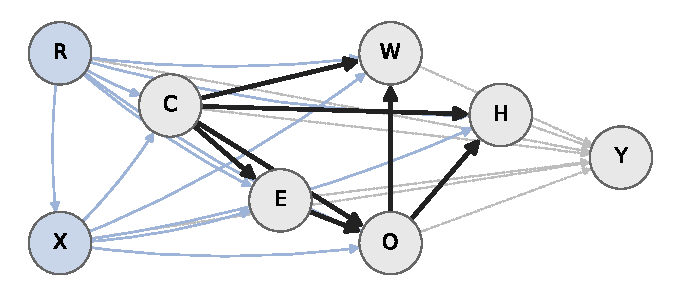
\includegraphics[width=\linewidth]{figures/bn_dag.pdf}\\[-1pt]
{\small (a) learned graph; blue: required $R,X$ edges}\end{minipage}\hfill
\begin{minipage}[b]{0.56\linewidth}\centering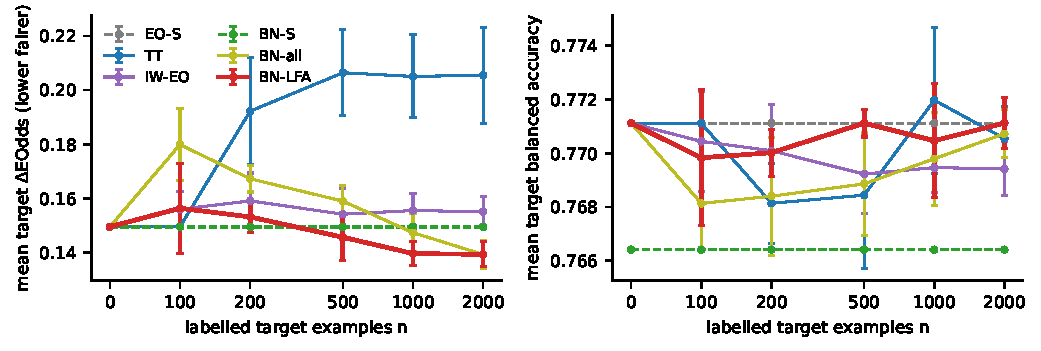
\includegraphics[width=\linewidth]{figures/budget_curves.pdf}\\[-1pt]
{\small (b) mean of 9 transfers; bars: s.d.\ over 5 seeds}\end{minipage}
\caption{(a) Structure learned in all six domains. (b) Target $\EO$ and balanced accuracy against the label budget.}
\label{fig:main}
\end{figure}
\begin{center}\small
\begin{tabularx}{\linewidth}{Xccc}
\toprule
Method & BA ($n$ = 200 / 1000) & $\EO$ ($n$ = 200 / 1000) & Log loss / Brier\\
\midrule
EO-S (source rule) & 0.771 / 0.771 & 0.150 / 0.150 & 0.448 / 0.147\\
TT (target thresholds) & 0.768 / 0.772 & 0.192 / 0.205 & 0.448 / 0.147\\
IW-EO (closest baseline) & 0.770 / 0.769 & 0.159 / 0.156 & 0.449 / 0.147\\
LR-T (target retraining) & 0.738 / 0.763 & 0.521 / 0.453 & 0.461 / 0.151\\
BN-all (ablation) & 0.768 / 0.770 & 0.167 / 0.147 & 0.445 / 0.146\\
BN-rand (ablation) & 0.771 / 0.770 & 0.165 / 0.152 & 0.447 / 0.146\\
BN-LL (ablation) & 0.770 / 0.772 & 0.150 / 0.143 & 0.445 / 0.146\\
\textbf{BN-LFA (proposed)} & 0.770 / 0.770 & \textbf{0.153 / 0.140} & 0.445 / 0.146\\
\bottomrule
\end{tabularx}
\end{center}
{\small \textbf{Table note:} means of 9 transfers $\times$ 5 seeds; BA higher, $\EO$ lower is better; log loss and
Brier at $n=1000$; target test splits of 20{,}681--39{,}551 persons; operating point $\delta=0.02$. Paired BN-LFA minus comparator, household-bootstrap 95\,\% CI, Holm $p$: TT $-0.039$
$[-0.045,-0.030]$ and $-0.065$ $[-0.070,-0.047]$ ($p=0.006$); BN-all $-0.014$ $[-0.020,-0.004]$ ($p=0.032$) and $-0.008$
$[-0.013,0.001]$ ($p=0.246$); IW-EO $-0.006$ $[-0.011,0.003]$ and $-0.016$ $[-0.022,0.001]$ ($p\ge0.22$). BA was
non-inferior in all six tests.}

\textbf{Main finding:} \emph{partially supported}. At matched utility (BA within 0.003), local adaptation beat spending
the labels on target thresholds at both budgets and beat updating every factor at $n=200$, but not covariate
reweighting; its gain over keeping the source rule was exploratory and not significant ($-0.010$ $[-0.018,0.004]$ at
$n=1000$). The source rule degraded little after zero-label transfer (mean $+0.028$, worst $+0.096$), leaving little to
repair.\\
\textbf{Mechanism and failure:} the diagnostic tracks the fairness change (predicted vs.\ observed change of the source
rule's gap over the nine pairs: Spearman 0.88, $p=0.002$, exploratory). State transfers mostly select education
$P(E\mid R,X,C)$ and the outcome factor; race composition is detected first but barely moves group error rates. Dropping
decision impact (0.143) or random factors (0.152) weakened BN-LFA (0.140) only slightly. At $n=200$, updating every
factor lowered held-out joint log-likelihood ($-8.926$ vs.\ $-8.898$ per person), BN-LFA raised it ($-8.873$). In the
synthetic study, BN-LFA with unlabelled covariates repaired a group-specific composition shift that IW-EO could not
(0.134 vs.\ 0.220; EO-S 0.241). It failed when three factors shifted (0.187 vs.\ 0.184 for EO-S), with coarse bins
(0.150 vs.\ 0.145) and when its top factor was excluded ($+0.009$).

\section{Limitations, ethics and conclusion}
The graph is associational and its tiers are assumptions; results describe the unweighted sample of three states and
two years (survey-weighted BN-LFA$-$TT averages $-0.072$, per-pair replicate SEs up to 0.066). Gaps are max$-$min
statistics over 7--10 groups; American Indian, Alaska Native and Pacific Islander cells are too small for any claim. The
nominal \$50k label ignores cost of living and encodes historical inequality, and group thresholds use race and sex,
which may be unlawful in practice. Conclusion: with few labels, adapting $\le2$ factors is a safer use of target data
than refitting thresholds, but here it offers no reliable gain over reweighting or no adaptation. Next: a third year.

\section*{Reproducibility and individual contributions}
\textbf{Reproduce:} \emph{Run all} in \texttt{problem5\_fairness\_transfer\_bn.ipynb} (Google Colab CPU, 13 min;
about 30 min on a 4-core laptop); settings: its \texttt{CFG} cell; versions in
\texttt{results/reproducibility.json}; headline table: \texttt{results/metrics/confirmatory\_tests\_holm.csv}.\\
\textbf{Aslam Mugutkhan}: \fillin{implementation/analysis artifacts and verification}.\\
\textbf{Rao Ashlesha Padmananda}: \fillin{implementation/analysis artifacts and verification}.\\
\textbf{Evidence:} \texttt{docs/requirements\_matrix.md}, \texttt{results/}.

\begin{thebibliography}{9}\footnotesize\setlength{\itemsep}{0pt}\setlength{\parskip}{0pt}
\bibitem{schrouff} J.~Schrouff, N.~Harris, S.~Koyejo et al. Diagnosing failures of fairness transfer across distribution
shift in real-world medical settings. NeurIPS 35, 2022.
\bibitem{census} U.S. Census Bureau. American Community Survey 1-Year PUMS, 2018 and 2019 person files.
\url{https://www2.census.gov/programs-surveys/acs/data/pums/}, accessed 30 Oct and 6 Nov 2026.
\bibitem{ding} F.~Ding, M.~Hardt, J.~Miller, L.~Schmidt. Retiring Adult: New datasets for fair machine learning.
NeurIPS 34, 2021. arXiv:2108.04884.
\bibitem{hardt} M.~Hardt, E.~Price, N.~Srebro. Equality of opportunity in supervised learning. NeurIPS 29, 2016.
\bibitem{pearl} J.~Pearl, E.~Bareinboim. Transportability of causal and statistical relations: A formal approach. AAAI
2011, 247--254.
\bibitem{shimodaira} H.~Shimodaira. Improving predictive inference under covariate shift by weighting the
log-likelihood function. J.\ Stat.\ Planning and Inference 90(2):227--244, 2000.
\bibitem{singh} H.~Singh, R.~Singh, V.~Mhasawade, R.~Chunara. Fairness violations and mitigation under covariate shift.
FAccT 2021.
\bibitem{rezaei} A.~Rezaei, A.~Liu, O.~Memarrast, B.~D.~Ziebart. Robust fairness under covariate shift. AAAI
35(11):9419--9427, 2021.
\bibitem{shao} M.~Shao, D.~Li, C.~Zhao, X.~Wu, Y.~Lin, Q.~Tian. Supervised algorithmic fairness in distribution shifts:
A survey. IJCAI 2024, 8225--8233.
\end{thebibliography}
\end{document}
